\documentclass[%
12pt,
twoside,
reprint,
amsmath,amssymb,
aps,
]{article}

%PDF Searchable copyable, fix symbols
\usepackage{cmap}
\usepackage[T1]{fontenc}

%Page numbers
\pagestyle{plain}

%Math Symbols
\usepackage{amsmath}
\usepackage{gensymb}
\usepackage{xfrac} %different fractions
\usepackage{bm} %bold

%Images
\usepackage{graphicx}
\usepackage{subfig}
\usepackage{caption}
\usepackage[export]{adjustbox} %scaling

%Tables
\usepackage{float,tabularx} %alternative table layout
\usepackage{dcolumn} %aligning decimals
\usepackage{makecell} %used for multi-line cells
\newcolumntype{Y}{>{\raggedleft\arraybackslash}X} %used with tabularx for sizing columns
\newcolumntype{Z}{>{\centering\arraybackslash}X}  %used with tabularx for sizing columns
\newcolumntype{?}{!{\vrule width 2pt}} %bold vertical line in table
\setlength{\extrarowheight}{5pt} %spacing between rows

%Text/paragraph formatting
\usepackage{indentfirst}
\usepackage{setspace} 
\usepackage{listings} %for displaying code
\usepackage{color, soul} %for highlighting text

%Shapes/geometries
\usepackage{tikz}
\usetikzlibrary{calc, shapes}

%Page formatting
\usepackage[margin=1in]{geometry}

%Table of Contents
\usepackage{hyperref}
\hypersetup{ %Hyplink to location
	colorlinks,
	citecolor=black,
	filecolor=black,
	linkcolor=black,
	urlcolor=black
}
%\usepackage[indentunnumbered]{unnumberedtotoc}

%Line Numbers
\usepackage{lineno}
\linenumbers

\begin{document}
	\thispagestyle{empty}
	\begin{center}
		\begin{minipage}{0.75\linewidth}
			\centering
			%Thesis title
			{\uppercase{\Large Development of a Low Energy Neutron Source for Bubble Chamber Calibrations\par}}
			\vspace{3cm}
			%Author's name
			{\Large Salvatore Zerbo \\ Advisor: Russell Neilson\par}
			\vspace{3cm}
			%Degree
			{\Large Submitted in partial fulfillment of the requirements for the degree of Bachelor of Science in Physics\par}
			\vspace{3cm}
			%Date
			{\Large Drexel University \\ Philadelphia, PA \\ June 2019\par}
			\vspace{2cm}
			\includegraphics[width=0.3\linewidth]{Images/logo.png}
		\end{minipage}
	\end{center}

	\pagebreak
	
	\tableofcontents
	
	\raggedbottom
	\pagebreak
	
	\phantomsection
	\begin{abstract}
	\addcontentsline{toc}{section}{Abstract}
	\doublespacing
	\par The use of bubble chambers for direct dark matter detection requires high sensitivity to energy levels in the range of 1-100 keV and strict measures to reduce background radiation. Neutrons can be used to simulate WIMP elastic scattering interactions with the target volume in order to ensure high detection efficiency. We aim to develop a low energy neutron source that will allow us to properly calibrate bubble chambers to ensure their ability to detect such events. We propose a solution consisting of a neutron source composed of a radioisotope capable of emitting gamma radiation at the required energy thresholds and a target capable of ejecting photoneutrons when struck by the gamma radiation. We have chosen seven main candidates for a gamma source, taking note of important properties such as half-life, availability, cost, and many others. We have also calculated the theoretical energies of the neutrons emitted by each source and the rate at which each source would emit neutrons. We utilize the GEANT4 simulation software to explore various scenarios and determine effective neutron emission rates and the energies upon interaction with the C$_{3}$F$_{8}$. Results yielded from the Drexel Bubble Chamber will be useful for other members of the PICO collaboration and other direct detection experiments. \hl{[include other results as they come along]}
	\end{abstract}
	
	\section{Introduction}
	\doublespacing
	\subsection{Dark Matter \& Bubble Chambers}
	\par The nature of cosmological dark matter has been an elusive mystery for many decades despite occupying nearly a quarter of the universe's content$^{\cite{1807.06209}}$. The modern theory of Weakly Interacting Massive Particles (WIMPs) requires highly specialized detection methods. WIMPs as the leading candidate address many critical issues in the $\Lambda$CDM Model such as galaxy rotation curves, the gravitational lensing of light in underdense regions, and the flatness of the universe$^{\cite{1303.2686}}$. 
	\par Bubble chambers have been used since the early 1950's as particle detectors$^{\cite{0604152}}$ and have more recently been adapted for the detection of WIMPs. Bubble chambers function by maintaining a liquid in a superheated state through tuning its temperature and pressure. Once in this state, any particle that deposits energy greater than the threshold energy will result in bubble nucleation. The PICO Collaboration uses the concept of bubble chambers with superheated fluorine-based liquids to provide some of the strongest constraints on the WIMP nucleon cross-sections as illustrated in Figure 1$^{\cite{1702.07666}}$.
	
	\begin{figure}
		\includegraphics[scale = 0.4, center]{Images/constraints.png}
		\caption{\label{tab:table-name} Latest spin dependent constraints on the WIMP-nucleon cross section from PICO-60$^{\cite{1902.04031}}$. Other results include the first blind exposure of PICO-60 C3F8 (thick blue), as well as limits from PICO-60 CF3I (thick red), PICO-2L (thick purple), PICASSO (green band), SIMPLE (orange), PandaX-II (cyan), IceCube (dashed and dotted pink), and SuperK (dashed and dotted black). \hl{Not sure if I should manually label legend like paper does.}}
	\end{figure}
	
	\par The ability to achieve low background is critical to direct detection methods of WIMPs. Several design decisions have been included to maximize detection efficiency and ensure accuracy of events. Fluorine based liquids are especially appealing as a target volume due to their insensitivity to gamma and beta particles$^{\cite{1601.03729}}$. The use of piezoelectric sensors allows for discrimination of alphas by acoustic analysis. Muons are eliminated through the use of a water tank containing PMT's. Reconstruction of events in the target volume allows for discrimination of neutron events due to bubble multiplicity. 
	\par Previous bubble chambers$^{\cite{1902.04031}}$ in the PICO collaboration utilized an up-side down design where the target volume was placed below a buffer fluid as seen in Figure 2a. This chamber faced many issues in the form of particulate falling down into the target volume and other issues at the water-target fluid interface. The Drexel Bubble Chamber is a prototype right-side up design that aims to remove these issues by flipping the design. In order to isolate the target volume, we use a sharp temperature gradient between the active and non-active regions of the chamber as seen in Figure 2b.
	\par The bubble chambers require calibrations with several types of sources to ensure that each particle is detected and identified correctly. Most importantly, we must be sure that the conditions of the chamber allow for detection of WIMPs. As result, the detector must be sensitive to elastic scattering interactions from nuclear recoils in energy ranges of 1-100 keV. The best method for determining the efficiency of nuclear recoils is through low energy neutron calibrations. 
	
	\begin{figure}[H]
		\centering
		\subfloat[]{{\includegraphics[scale = 0.55]{Images/pico60.png} }}%
		\qquad
		\subfloat[]{{\includegraphics[scale = 0.55]{Images/dbctext.png} }}%
		\caption{\label{tab:table-name} (a) Design of PICO-60 bubble chamber. This design places the target volume below a water buffer layer. (b) CAD design of the right-side up Drexel Bubble Chamber.}%
	\end{figure}
	
	\subsection{Low Energy Neutrons}
	\par Neutrons can be generated through many different methods such as spontaneous fission, $\alpha$ interactions on a low-atomic-weight target, $\gamma$ interactions with a target such as $^{9}$Be or $^{2}$D, or through neutron generators. We desire to generate neutrons at relatively low ($\leq$ 200 keV) energy scales, and as a result, the only viable method for a neutron source is through $\gamma$ interactions upon a target. Although the other methods may satisfy many of the requirements, they are only capable of producing neutrons on the MeV energy scale, which is a vital component to this project. We require low energy neutrons to properly calibrate bubble chambers for WIMP events which will occur at similar energy levels. Without neutron calibration, it is impossible to tell if the chambers are able to efficiently and accurately detect potential WIMP events.
	\par Neutron sources for chamber calibrations have been considered before within the PICO collaboration$^{\cite{internalalv}-\cite{robinson}}$; however, a low energy neutron source has yet to be developed. The components of our neutron source will include a gamma source, target material, and appropriate shielding to prevent gammas and neutrons from leaking in undesired directions. Starting with an isotope that undergoes some form of decay, it will then emit gammas at a monoenergetic level. If the gamma contains more energy than the threshold for neutron production, it will deposit enough energy upon contact and emit a neutron. The neutron will then come into contact with the bubble chamber and deposit its energy on to superheated C$_{3}$F$_{8}$. From there, our chamber will detect an event trigger, and we will be able to perform calibrations through image analysis, piezoelectric acoustic data, and other simulations.
	
	\begin{equation}
	\begin{aligned}	
	^{9}Be + \gamma \longrightarrow\ ^{8}Be + n \\
	^{2}D + \gamma \longrightarrow\ ^{1}D + n
	\end{aligned}
	\end{equation}
	
	\par Equation 1 shows the reactions of the targets with an incident gamma and the resulting isotopes and particles. From this equation, we are able to determine the threshold energy of the gammas needed to emit one neutron from each nucleus with simple conservation of energy. Since the number of electrons does not change during this process, we are free to emit them from the calculations since they will cancel. A similar calculation for $^{2}D$ is omitted, but yields 2.23 MeV. For the $^{9}Be$ target, we have
	
	\begin{equation}
	\begin{aligned}	
	m_{^{9}Be} * c^{2} + Q = m_{^{8}Be} * c^{2} + m_{n} * c^{2} \\
	\Rightarrow Q = (m_{^{8}Be} + m_{n} - m_{^{9}Be}) * c^{2} = 1.67\ MeV
	\end{aligned}
	\end{equation}
	
	\par The key difficulty in designing a low energy neutron source is finding an isotope that fits all of our requirements. The isotope must have a long enough half-life such that it can survive through the extensive safety procedures at Snolab without losing a majority of the material. It should also produce gammas close to the threshold energy of the target such that the emitted neutron will be in our desired energy range. It is important to have large branching ratios for these gamma energies so that we obtain neutrons primarily at the energy we desire. Finally, the isotope should be feasible to buy in large enough quantities without either costing too much or requiring too much time to be delivered.
	
	\section{Methods}
	\subsection{Identifying the Proper Gamma Source}
	\par Our first approach to tackling this problem is to create an exhaustive list of all potential candidates for gamma sources and note the specific properties that we require them to have. Included in the list will be each candidates gamma energy spectrum, branching ratios, half-life, and other information on the feasibility of acquiring the isotope. Another important property to keep track of is the neutron production rate. If the rate is too low, then we will not be able to perform accurate calibrations; however, we also want to avoid too many neutrons from being produced, as this could cause unwanted leakage that could cause issues elsewhere.
	\par By searching the Table of Isotopes, a list has been developed as seen below in Table 1. The seven isotopes listed are the most likely in terms of their branching ratios, gamma energies, half-lives, and feasibility of being obtained. Most gamma sources do not emit >2 MeV, so finding a source to use with a $^{2}$D target is unlikely outside of $^{226}$Ra. 	
		
	\begin{table}
		\begin{center}
		\scriptsize
		\begin{tabular}{l l l l l l}
			\hline
			\textbf{Isotope} & \textbf{Target} & \textbf{Half-Life (Years)} & \makecell{\textbf{Main Gamma} \\ \textbf{Energy (keV)}} & \textbf{Branching Ratios (\%)} \\ \hline
			$^{26}$Al            & $^{9}$Be           & 7.17E+05                   & 1808                             & 99.76                          \\ \hline
			$^{207}$Bi           & $^{9}$Be          & 31.55                      & 1770                             & 6.87                           \\ \hline
			$^{58}$Co            & $^{9}$Be            & 0.19                       & 1674                             & 0.52                           \\ \hline
			$^{150}$Eu           & $^{9}$Be           & 36.9                       & 1690                             & 0.15                           \\ \hline
			$^{124}$Sb           & $^{9}$Be           & 0.16                       & 1690                             & 47.79                          \\ \hline
			$^{88}$Y             & $^{9}$Be            & 0.29                       & 1836                             & 99.2                           \\ \hline
			$^{226}$Ra($^{214}$Bi)       & $^{2}$D              & 1590                       & 2447                             & 1.57                           \\ \hline
		\end{tabular}
		\caption{\label{tab:table-name} Lists of potential gamma radioisotope sources with their corresponding targets, half-lives, relevant gamma energies, and branching ratios gathered from the Table of Isotopes.}
	\end{center}
	\end{table}
		
	\subsection{Calculations}
	\par After gathering the list of potential gamma sources, our next step is to calculate and gather as much information about each of the isotopes to better inform our decision. This data is listed below in Table 2. The expected theoretical neutron energies for each system is calculated through$^{\cite{wattenberg}}$:
	
	\begin{equation}
	\begin{array}{c}
	E_{n} = \frac{A - 1}{A} [E_{\gamma} - Q - \frac{E_{\gamma}^{2}}{1862 (A - 1)}] + \delta; \\
	\end{array}
	\end{equation}
	
	Here, A is the mass number, $E_{\gamma}$ is the energy of the incident gamma, Q is the threshold energy for the target, and $\delta$ is an energy spread function defined by:
	
	\begin{equation}
	\begin{array}{c}
	\delta \approx E_{\gamma}[\frac{2(A-1)(E_{\gamma}-Q)}{931A^{3}}]^{\sfrac{1}{2}} cos(\theta) \\
	\delta_{max} = 2E_{\gamma}[\frac{2(A-1)(E_{\gamma}-Q)}{931A^{3}}]^{\sfrac{1}{2}}
	\end{array}
	\end{equation}
	
	The angle $\theta$ is defined as the angle between the incident gamma and the emitted neutron. As seen in Figure 3, the $\theta$ dependence of $\delta$ can have significant effects, and it is difficult to determine the value of $\theta$, so we will place the gamma source such that the gammas are incident in an isotropic manner, yielding $\delta_{max}$ instead. 
	
	\begin{figure}
		\includegraphics[scale = 0.7, center]{Images/theta_distribution.png}
		\caption{\label{tab:table-name} Expected neutron energies over a range of incident gamma angles from 0 to 2$\pi$. This is shown for each of our potential sources. Some like $^{214}$Bi have large variability while most only vary by a few keV.}
	\end{figure}
	
	\par A much more involved process is estimating the rate at which neutrons will be emitted from each system. We first start with basic assumptions that will allow for convenience when doing the calculations: we will have 1g of material for both the gamma source and target, and the distance between the source and target will be 1cm. From the half-life of the gamma source, the decay constant, and subsequently, the activity can be calculated:
	
	\begin{equation*}
	t_{1/2} = \frac{ln(2)}{\lambda} \implies \lambda = \frac{ln(2)}{t_{1/2}}
	\end{equation*}
	\begin{equation*}
	A = \lambda N
	\end{equation*}
	
	\begin{table}
		\begin{center}
			\scriptsize
			\begin{tabular}{p{3.1cm} p{3.1cm} p{3.1cm}}
				\hline
				\textbf{Isotope} & \textbf{Theoretical Neutron Energy (keV)} & \textbf{n/s/g} \\ \hline
				$^{26}$Al &\ \ \ \ \ \ \ \ \ \ 128.99 & 539 \\ \hline
				$^{207}$Bi &\ \ \ \ \ \ \ \ \ \ 94.14 & 1.52E+05 \\ \hline
				$^{58}$Co &\ \ \ \ \ \ \ \ \ \ 4.42 & 2.27E+07 \\ \hline
				$^{150}$Eu &\ \ \ \ \ \ \ \ \ \ 19.93 & 2.51E+04 \\ \hline
				$^{124}$Sb &\ \ \ \ \ \ \ \ \ \ 19.93 & 2.07E+09 \\ \hline
				$^{88}$Y &\ \ \ \ \ \ \ \ \ \ 154.62 & 3.34E+08 \\ \hline
				$^{226}$Ra($^{214}$Bi) &\ \ \ \ \ \ \ \ \ \ 144.25 & 9.00E+03 \\ \hline
			\end{tabular}
			\caption{Gamma sources with their corresponding expected neutron energies and neutron rates.}
		\end{center}
	\end{table}
	
	\noindent Then the number of neutrons can be estimated through the most relevant factors: activity, branching ratio, the amount of target, the gamma-neutron cross section, and the spherical surface area covered by the isotropic emission of gammas. The gamma-neutron cross section can be found by reading them off plots from JANIS for each specific incident gamma energy. Combining these factors leads to equation 5:
	
	\begin{equation}
	\#n \approx A * \% Branching * \frac{m_{target}}{m_{target\ nucleus}} * \sigma * \frac{1}{SA_{sphere}}
	\end{equation}
	
	\par Two more calculations were done to determine how much deuterium is found per amount of heavy water since that is the most available form and how large would a sphere of that amount of heavy water be. The first is simply calculated by taking the ratios of the masses, so if we desire 1g of Deuterium as was used for the calculations above, we would need 10g of heavy water. The size of a sphere would then be found by equating the mass to the density times the volume of a sphere. This yields a radius of 1.29 cm, which is on the scale of the size that we would like the system to be at.
	
	\subsection{Choosing a Source}
	\par The availability of our seven potential sources has been determined based on the strength, price, lead time, and supplier. The first isotope to be explored is $^{26}$Al, which looks to be a strong candidate at first; however, it is incredibly difficult and expensive to obtain. Only one supplier, Oak Ridge National Laboratory, is able to provide it at a cost of \$381 per nCi. This is incredibly expensive considering we require amounts on the scale of mCi for a neutron rate large enough. $^{150}$Eu is extremely is rare, making it infeasible to use for a gamma source. Similarly, $^{58}$Co is also expensive and rare, requiring too long of a lead time to acquire.
	\par Of the remaining sources, $^{226}$Ra is the weakest due to the available strength of the source and high theoretical neutron energy. This leaves the two most popular gamma sources, $^{88}$Y and $^{124}$Sb, and $^{207}$Bi. Looking at Table 1, it's clear that $^{124}$Sb will never make it through the Snolab safety procedures and would be replaced far too often, resulting in high expenses. $^{88}$Y, although a strong contender, has been studied before and does not result in low neutron energies that we would like. As result, we are able to conclude that the best source for our purposes will be $^{207}$Bi.
	
	\subsection{Improved Neutron Rates}
	\par The calculations done above for the neutron rates were naive in a few ways. First, we assumed that we would have 1g of gamma source material, when it would be more proper to use the the quoted strength of the gamma sources instead. The target was approximated as a sphere, when it will actually be a cylinder. In addition, the target was assumed to be homogeneous and the mass was severely underestimated. In order to correct for this, we improve upon the calculations below.
	\par The easiest issue to correct is that of the amount of gamma source material. The strengths quoted in Table 1, when multiplied by a scaling factor of 3.7E5, will replace A in Equation 5. Next, the actual target that will be used is BeO, which given a density of $3.02 \sfrac{g}{cm^{3}}$ and the dimensions in Figure 4b, yields a target mass of 29.15g. An additional factor of $\sfrac{9}{25}$ will be picked up in Equation 5 due to the inhomogeneity of the target.
	\par A better estimation of the neutron rate can be found from taking the average value of the function:
	
	\begin{figure}
		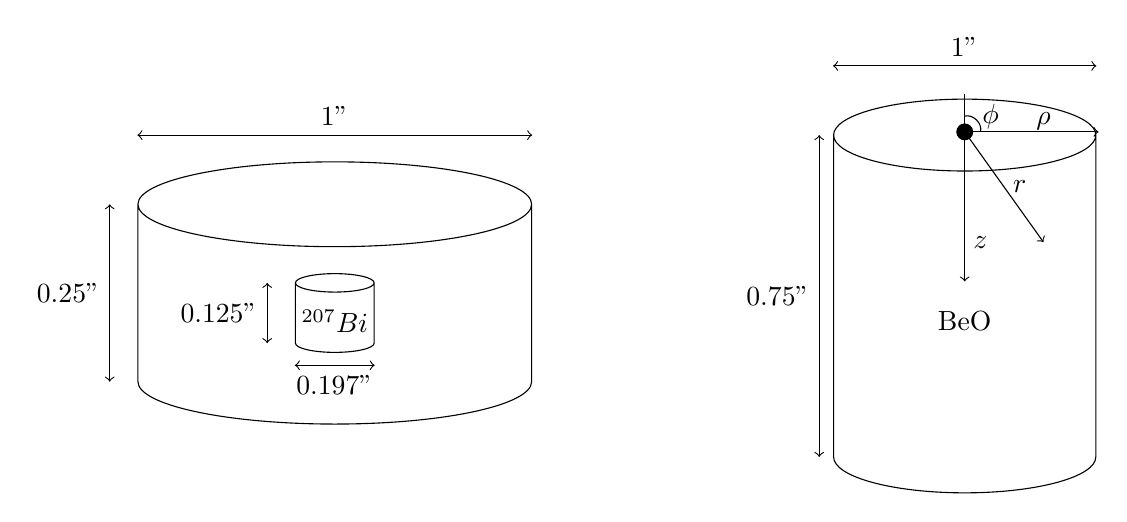
\begin{tikzpicture}[scale=1]	
		\node (c1) [cylinder, shape border rotate=90, draw,minimum height=3.33cm,minimum width=5cm] {$^{207}Bi$};
		
		\node (c) [cylinder, shape aspect = 1, shape border rotate=90, draw,minimum height=1cm,minimum width=1cm] {};
		
		\draw [<->] ([yshift=25]c1.before top) -- ([yshift=25]c1.after top) node [midway, above,fill=white] {$1"$};
		\draw [<->] ([yshift=-8]c.before bottom) -- ([yshift=-8]c.after bottom) node [midway, below] {$0.197"$};
		\draw [<->] ([xshift=-10pt]c.after bottom) -- ([xshift=-10pt]c.before top) node [midway, left] {$0.125"$};
		\draw [<->] ([xshift=-10pt]c1.after bottom) -- ([xshift=-10pt]c1.before top) node [midway, left] {$0.25"$};
		
		\node (A) [cylinder, shape border rotate=90, draw,minimum height=5cm,minimum width=3.33cm]
		at (8, 0, 0){BeO};
		\filldraw [fill](8, 2.4) circle (0.1 cm);
		\draw [->] (8, 2.4) -- (9, 1);
		\draw [->] (8, 2.4) -- (9.7, 2.4);
		\draw [->] (8, 2.4) -- (8, 0.5);
		\draw[-] (8, 2.4) -- (8, 2.88);
		\draw [-] (8.2, 2.4) to [bend right=60] node {} (8, 2.6);
		
		\node[] at (9, 2.53) {$\rho$};
		\node[] at (8.7, 1.7) {$r$};
		\node[] at (8.2, 1) {$z$};
		\node[] at (8.33, 2.6) {$\phi$};
		
		\draw [<->] ([yshift=25]A.before top) -- ([yshift=25]A.after top) node [midway, above,fill=white] {$1"$};
		\draw [<->] ([xshift=-5pt]A.after bottom) -- ([xshift=-5pt]A.before top) node [midway, left] {$0.75"$};
		\end{tikzpicture}
		\caption{\label{tab:table-name}(a) Dimensional drawing of the $^{207}$Bi source. The source consists of an active volume located inside a non-active disk. (b) Dimensional drawing of the gamma target, BeO. Integrating over this volume allows for more accurate calculations.}
	\end{figure}
	
	\begin{equation}
	\begin{aligned}
	\bar{f} = \frac{1}{V} \iiint_D f(\rho, \phi, z) dV
	\end{aligned}
	\end{equation}
	
	\noindent Applying Equation 6 to our function in Equation 5 yields:
	
	\begin{equation}
	\begin{aligned}
	\#n \approx A * \% Branching * (\frac{m_{target}}{m_{Be}} * \frac{9}{25}) * \sigma * \frac{1}{V} \int_{0}^{1.905}\int_{0}^{2 \pi}\int_{0}^{1.27} \frac{\rho}{4*\pi*r^{2}} d\rho d\phi dz
	\end{aligned}
	\end{equation}
	
	\noindent Here, $\rho = \sqrt{(r^{2} + z^{2})}$, V is the volume of the cylinder in Figure 4b, and the additional mass factor has been included. The updated rates can be seen below in Table 3, and as a sanity check, we can compare our calculated rates with other results. For 1 Ci of $^{88}$Y, the expected value is 10E4 N/s/Ci$^{\cite{1601.03729}}$. For 0.1 mCi, we would expect a rate on the order of 10 n/s, and our calculations yield 25.89 n/s. More importantly, the new estimated neutron rate for $^{207}$Bi is 0.30 n/s.

	\section{Analysis}
	\subsection{Simulations}
	\noindent \hl{[maybe this should be in methods too?]}
	\par GEANT4 is a simulation software that allows for the tracking of particles as they pass through matter, recording properties of each event such as the volume collided with, energies of the particle, scattering types, and more. GEANT4 is highly versatile in its ability to simulate particle events for a wide array of purposes ranging from astroparticle physics to accelerator physics. The software allows for highly detailed and specialized construction of detectors, enabling for high accuracy simulations of many different scenarios.
	
	\begin{figure}[H]
		\includegraphics[scale = 0.42, center]{Images/histogram_distancetest.png}
		\caption{\label{tab:table-name} GEANT4 simulations overplotted to show the number of events in the target volume and the average energy of those events. These simulations were at varying distances from the center of the target volume. At 100mm, the source was placed far from the detector; at 58mm, the source was placed right outside the mineral oil; and at 16mm, the source was placed inside the mineral, right up against the C$_{3}$F$_{8}$.}
	\end{figure}
	
	\par Our first test with GEANT4 is to gather neutron deposition energies at varying distances. The three potential locations that the neutron source can be placed at are far outside the chamber, up against the mineral oil, or up against the C$_{3}$F$_{8}$. The results of the simulations can be seen above in Figure 5. It is clear that a source placed as close as possible results in the greatest number of hits and the highest average energy upon recoil. The differences in the results between distances is inflated by the mineral oil. Mineral oil is a strong shield against neutrons, greatly reducing both the energies and counts of neutrons that reach the target volume.
	
	\noindent \hl{[Probably replace these histograms with better simulation plots]} \\
	\hl{[Need to fix scaling issues]}
	
	\begin{figure}[H]
		\includegraphics[scale = 0.45, center]{Images/histogram_particle_guide.png}
		\caption{\label{tab:table-name} GEANT4 simulations overplotted to show the number of events in the target volume and the average energy of those events. These simulations were run with a particle guide made of air, lead, and copper introduced inside the mineral oil volume.}
	\end{figure}

	\par Our second test is to determine whether placing a particle guide inside the mineral oil to allow for a clearer path for the neutrons to traverse towards the C$_{3}$F$_{8}$. Inserting and removing the source from the mineral is a tedious task with a small chamber like the DBC, so it will be exponentially more difficult for the large chambers. We test with three different materials of air, copper, and lead. Looking at Figure 6, we see, as expected, that air performs the best at allowing neutrons to travel through it. Even in the best case scenario, a particle guide performs significantly worse than placing the source inside the mineral oil.

	\par In order to ensure that our simulations are correct, we simulate a $^{244}$Cm source and compare with data obtained from the DBC. From the data collected, the source should emit neutrons at approximately 1.8 n/s, and we should see a bubble rate peaking at 100 bubbles/hr for a 2 keV threshold.
	
	\noindent \hl{[write more once the cm244 simulations are fixed, also replace the plots too]}

	\begin{figure}[H]%
		\centering
		\subfloat[]{{\includegraphics[scale = 0.15]{Images/histogram_cm244.png} }}%
		\qquad
		\subfloat[]{{\includegraphics[scale = 0.15]{Images/energy_spectrum.png} }}%
		\caption{\label{tab:table-name} (a) Neutron energy counts when interacting with the target volume. Neutrons are emitted from $^{244}$Cm source directly above the chamber. (b) Emission energy spectrum of $^{244}$Cm from GEANT4.}%
	\end{figure}

	\subsection{Results}
	\hl{[fill this in once actual data is collected]}
	
	\section{Conclusion}
	\hl{[fill this in once data collection finished]}
	
	\subsection{Future Plans}
	\hl{[fill this in once at end of spring term]}
	
	\pagebreak
	\phantomsection
	\noindent \hl{[make sure everything in references is properly cited]}
	\begin{thebibliography}{1}
		\addcontentsline{toc}{section}{References}
		\bibitem{1807.06209} N. Aghanim et al. (Planck Collaboration). 2018. Planck 2018 results. VI. Cosmological parameters. arXiv:1807.06209 
		\bibitem{1303.2686} J. I. Collar. 2017. Applications of an $^{88}$Y/Be photo-neutron calibration source
		to Dark Matter and Neutrino Experiments. arXiv:1303.2686
		\bibitem{0604152} G. Giacomelli. 2006. Introduction to the Workshop "30 years of bubble chamber physics". arXiv:0604152
		\bibitem{1702.07666} C. Amole et al. (PICO Collaboration). 2017. Dark Matter Search Results from the PICO-60 C$_{3}$F$_{8}$ Bubble Chamber. arXiv:1702.07666 
		\bibitem{1601.03729} C. Amole et al. (PICO Collaboration). 2016. Improved dark matter search results from PICO-2L Run 2. arXiv:1601.03729
		\bibitem{1902.04031} C. Amole et al. (PICO Collaboration). 2019. Dark Matter Search Results from the  Complete Exposure of the PICO-60 C$_{3}$F$_{8}$ Bubble Chamber. arXiv:1902.04031 
		\bibitem{internalalv} Alvaro E. Chavarria. 2012. Calibrating the energy response of bubble chambers to $^{19}$F recoils by taking advantage of the elastic scattering resonances. (PICO Internal Document).
		\bibitem{internalamole} C. Amole et al. (PICO Collaboration). 2018. Measurements and models of the efficiency of bubble nucleation by nuclear and electron recoils in superheated liquids. (PICO Internal Document).
		\bibitem{robinson} A. Robinson. 2015. Photoneutron Source Characterization and Neutron Simulations.
		\bibitem{wattenberg} A. Wattenberg. Photo-Neutron Sources. Preliminary Report No. 6. United States: N. p., 1949. Web. doi:10.2172/4448374.
		\bibitem{janis} N. Soppera, M. Bossant, E. Dupont, "JANIS 4: An Improved Version of the NEA Java-based Nuclear Data Information System", Nuclear Data Sheets, Volume 120, June 2014, Pages 294-296.
		\bibitem{chen} Chen, J., \& Savage, M. J. (1999). np$\rightarrow$d$\gamma$ for big-bang nucleosynthesis. Physical Review C, 60(6) doi:10.1103/PhysRevC.60.065205
		
	\end{thebibliography}
	\section*{Appendix A: GEANT4 Detector Construction}
	\addcontentsline{toc}{section}{Appendix A: GEANT4 Detector Construction}
	\noindent \hl{[maybe move this text to simulations section]}
	\par The current model of the Drexel Bubble Chamber is simulated using a simplistic version of the detector. Within GEANT, the world is composed of volume of air surrounding the detector, which has four components. The outer most layer is a cylindrical container of acrylic, and the next layer within is a similarly shaped object used for the mineral oil. The next object located within the mineral oil is the quartz container for the inner most volume, the C$_{3}$F$_{8}$. The C$_{3}$F$_{8}$ volume is set as the sensitive detector so that when neutrons scatter off the volume, GEANT will record the data. \\
	\hl{[might not need all these images]} \\
	\hl{[fix the color issues and reformat the layout]}
	\begin{figure}[H]%
		\centering
		\subfloat[]{{\includegraphics[scale = 0.2]{Images/dbc_geant.png} }}%
		\qquad
		\subfloat[]{{\includegraphics[scale = 0.2]{Images/particle_guide.png} }}%
		\qquad
		\subfloat[]{{\includegraphics[scale = 0.2]{Images/new_design.png} }}%
		\caption{\label{tab:table-name} (a) GEANT4 assembly of the relevant Drexel Bubble Chamber volume. The components are colored as: acrylic: cyan, mineral oil: red, quartz: white, C$_{3}$F$_{8}$: yellow. The yellow outer lines define the world of the system, which is given air as a material. (b) The brown material is the inclusion of a particle guide to aid in the neutrons traversing the mineral oil. (c) New design with top pieces constructed.}%
	\end{figure}

	\begin{figure}[H]%
		\centering
		\subfloat[]{{\includegraphics[scale = 0.24]{Images/16mm.png} }}%
		\qquad
		\subfloat[]{{\includegraphics[scale = 0.24]{Images/58mm.png} }}%
		\qquad
		\subfloat[]{{\includegraphics[scale = 0.24]{Images/100mm.png} }}%
		\caption{\label{tab:table-name} \hl{[replace this with single image showing each location]} (a) Neutron source located at 16mm away, inside the mineral oil. (b) Neutron source located 58mm away right outside the mineral oil. (c) Neutron source located far away from the chamber.}%
	\end{figure}

	\section*{Appendix B: $\gamma$-neutron Cross Section Plots}
	\addcontentsline{toc}{section}{Appendix B: $\gamma$-neutron Cross Section Plots}
	
	\begin{figure}[H]
		\includegraphics[scale = 2.5, center]{Images/be_plot.png}
		\caption{\label{tab:table-name} Cross sections for gamma-neutron interactions with a $^{9}$Be target as a function of incident gamma energies. Highlighted are the energies of the emitted gammas from each potential source$^{\cite{janis}}$.}
	\end{figure}

	\begin{figure}[H]
		\includegraphics[scale = 1.8, center]{Images/deuterium_cross_section.png}
		\caption{\label{tab:table-name} Cross sections for gamma-neutron interactions with a Deuterium target as a function of incident gamma energies. The energy for $^{226}$Ra is highlighted$^{\cite{chen}}$.}
	\end{figure}

	\makebox[12cm][c]{Advisor Signature: \makebox[5cm][c] {\hrulefill} \hfill}

\end{document}